\documentclass[11pt]{article}
\usepackage{latexsym}
\usepackage{amsmath}
\usepackage{amssymb}
\usepackage{amsthm}
\usepackage{epsfig}
\usepackage[tight]{subfigure}

\usepackage{amsmath}
\usepackage{hyperref}
\usepackage[table]{xcolor}

\DeclareMathOperator*{\minimize}{min}
\DeclareMathOperator*{\maximize}{max}
\DeclareMathOperator*{\argmax}{arg\,max}
\DeclareMathOperator*{\argmin}{arg\,min}

\usepackage{algorithm, algpseudocode}
 %on linux you may need to run sudo apt-get install texlive-full to install algorithm.sys

\usepackage{verbatim}

\newcommand{\handout}[5]{
  \noindent
  \begin{center}
  \framebox{
    \vbox{
      \hbox to 5.78in { {#1} \hfill #2 }
      \vspace{4mm}
      \hbox to 5.78in { {\Large \hfill #5  \hfill} }
      \vspace{2mm}
      \hbox to 5.78in { {\em #3 \hfill #4} }
    }
  }
  \end{center}
  \vspace*{4mm}
}

\newcommand{\lecture}[5]{\handout{#1}{#2}{#3}{#4}{#5}}
\newcommand{\collision}[0]{\mathrm{collision}}
\newcommand{\nocollision}[0]{\overline{\collision}}

\newcommand*{\QED}{\hfill\ensuremath{\square}}

\newtheorem{theorem}{Theorem}
\newtheorem{corollary}[theorem]{Corollary}
\newtheorem{lemma}[theorem]{Lemma}
\newtheorem{observation}[theorem]{Observation}
\newtheorem{proposition}[theorem]{Proposition}
\newtheorem{definition}[theorem]{Definition}
\newtheorem{claim}[theorem]{Claim}
\newtheorem{fact}[theorem]{Fact}
\newtheorem{assumption}[theorem]{Assumption}
\newtheorem{note}[theorem]{Note}

% 1-inch margins, from fullpage.sty by H.Partl, Version 2, Dec. 15, 1988.
\topmargin 0pt
\advance \topmargin by -\headheight
\advance \topmargin by -\headsep
\textheight 8.9in
\oddsidemargin 0pt
\evensidemargin \oddsidemargin
\marginparwidth 0.5in
\textwidth 6.5in

\parindent 0in
\parskip 1.5ex
%\renewcommand{\baselinestretch}{1.25}

\begin{document}

\lecture{Statistical Techniques in Robotics (16-831, S22)}{Lecture \#25
  (Wednesday, Apr 20)}{Lecturer: Kris Kitani}{Scribes: Siqi Chai, Jiajie Xu (Group A)}{Maximum Entropy IRL and Matrix Game IRL}

\section{Review}
In the previous lecture, we discussed Max Margin IRL. It relates the active imitation learning problem to max margin classifier problem. We also talked about Max-Margin Planning, but didn't finish this topic.

\subsection{Policy Value and Expected Policy Features}
We define policy value $V(\pi)$ (or equivalently $\mathbb{E}[V^\pi(s)]$) as:
\begin{align*}
V(\pi) &= \mathbb{E}_p \left[ \sum_{t=0}^\infty \gamma^t r(s_t) \right] \\
 &= \boldsymbol\theta \cdot E\left[ \sum_{t=0}^\infty \gamma^t \phi(s_t) \right] && \triangleright \phi(s_t)\text{ is features at each state} \\
 &= \boldsymbol\theta \cdot \boldsymbol\mu(\pi)
\end{align*}
We name $\boldsymbol\mu(\pi)$ expected feature counts. From the above equation, we know that policy value is linear in expected features. $\boldsymbol\mu(\pi)$ is an expected value over all possible trajectories and all possible states, it doesn't depend on a single state.

\subsection{Max Margin IRL}
Using the linearity above, we rewrite the policy value comparison between expert and other policy:
\[ \boldsymbol\theta \cdot \boldsymbol\mu(\pi^*) \geq \boldsymbol\theta \cdot \boldsymbol\mu(\pi) \]
Transfer this inequality into a max margin optimization problem with L2 regularization:
\begin{align*}
    \min_{\theta, t} \quad & \lambda \lVert\theta\rVert_2 -t \\
    \textrm{s.t.} \quad & \theta^\intercal (\mu(\pi^*)-\mu(\pi_n)) \geq t \quad \forall \pi_n \in \Pi
\end{align*}
where $\Pi$ is a finite set of competitive policies other than expert. This format of optimization is exactly the same as a max-margin classifier (SVM). Substitute $ t = \sum_i 1-\xi_i $ we get:
\begin{align}
\label{eq: maxmargin_irl}
    \min_{\theta, \xi} \quad & \lambda \lVert\theta\rVert_2 + \sum_i \xi_i \\
    \textrm{s.t.} \quad & \theta^\intercal (\mu(\pi^*)-\mu(\pi_i)) \geq 1-\xi_i \quad \forall i
\end{align}
We call the 1 margin, and $\xi_i$ slack as in the soft SVM setting. Then we can use quadratic programming to solve this optimization.

\begin{algorithm}
\caption{MaxMargin IRL}
\label{alg:maxmargin}
\begin{algorithmic}[1]
\Function {MaxMargin IRL}{$\mu(\pi^*)$}
\State $\Bar{\boldsymbol\mu}_D = \text{CountFeatures} (\mathcal{E}, \pi^*)$
\For {$i = 1 \cdots $}
    \State $\hat{\pi} = \mathop{argmax}_\pi \theta^\intercal \mu(\pi)$ \Comment{Solve RL to get competitive policy}
    \State $\mu(\hat{\pi_i}) = \mathbb{E}\left[ \sum_{t=0}^\infty \gamma^t \phi(s_t) \right]$ \Comment{Pre-compute feature count using MC roll out}
    \State $\theta = \text{QuadProg}(\lambda, \mu(\pi^*), \{ \mu(\hat{\pi}_n) \}_{n=1}^i)$ \Comment{update $\theta$ using quadratic programming, gradient descent, etc.}
\EndFor \\
\Return $\theta$
\EndFunction
\end{algorithmic}
\end{algorithm}

\subsection{Maximum Margin Planning}
Structured Output Max-Margin IRL (aka Maximum Margin Planning) is an algorithm built up on Max Margin IRL, and it can be used in different real robotics tasks instead of toy examples.

Define new quantities:
\begin{itemize}
    \item Cumulative Feature count from policy and trajectory: $\mu(\pi) \quad \mu(\zeta)$
    \item Feature map, features for each state-action pair: $F \in \mathbb{R}^{N \times |S||A|}$
    \item Occupancy measure: visitation count of each state-action pair: $\eta(a,s) \in \mathbb{R}^{|S||A|}$
    \item Relation: $\mu = F \eta$
\end{itemize}

Starting from equation (\ref{eq: maxmargin_irl}), we make the margin depend on the "distance" between policies:
\begin{align*}
    \min_{\theta, \xi} \quad & \lambda \lVert\theta\rVert_2 + \sum_i \xi_i \\
    \textrm{s.t.} \quad & \theta^\intercal (\mu(\pi^*)-\mu(\pi_i)) \geq \ell(\pi^*, \pi_i)-\xi_i \quad \forall i
\end{align*}

Through a lot of math, we can derive the final object function for Max-Margin planning:
\[ \min_{\theta} \frac{1}{2}||{\theta}||^2 + \lambda \sum_d \left\{ ({\theta}^\intercal F_d + l_d^\intercal)\eta_d^* - \theta^\intercal F_d \eta_d \right\} \]
which is the form of SVM with hinge loss, and we can use online sub-gradient descent to solve it.


\clearpage
\section{Summary}
\subsection{Maximum Entropy IRL}
In this class, we introduce a new algorithm under inverse reinforcement learning, called Maximum Entropy (MaxEnt) IRL. We use a different method related to entropy to set up objective function, instead of comparing value functions between expert and other competitive policy. In all previous methods, we assume linearization of reward function, now we don't make this assumption, but it will emerge as part of the derivation.

We want to estimate the distribution over all possible state trajectories generated by Markov decision process, $p(\zeta)$, which is huge and often infinity in size. As we have no data/evidence from this distribution, we consider every trajectory to be equally likely (a uniform distribution). This comes from the idea of Occam's razor, we look for the simplest explanation, which is most likely to be true.

\subsubsection{Information Entropy and Objective Function}
The definition of information entropy is central to the derivation of MaxEnt IRL. Recall, the entropy of a discrete distribution is:
\[ \mathcal{H}(x) = -\sum_x p(x) \log(p(x)) \]
Entropy for a continuous distribution:
\[ \mathcal{H}(x) = -\int_x p(x) \log(p(x)) dx \]
Entropy measures the uncertainty of the distribution. The more information we get about $x$ from distribution, the lower entropy it has. A simple example to understand this is the entropy of binomial random variable:
\[ \mathcal{H}(x) = -(x \log_2x) - (1-x) \log_2(1-x) \]
\begin{figure}[H]
    \centering
    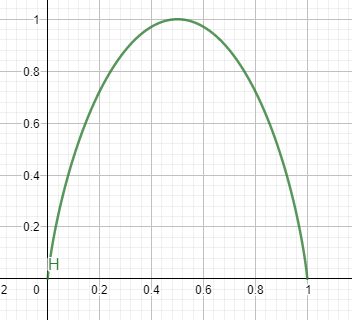
\includegraphics[width=0.25\textwidth]{pic-s3/binary_entropy_function.png}
\end{figure}
This entropy takes maximum when probability of $x=1$ is 0.5. Intuitively for our trajectory distribution, when it is a uniform distribution, the entropy is maximized.

Maximizing entropy is the same as minimizing negative entropy, therefore our objective function is:
\[ \mathop{min}_{p(\zeta)} \sum_{\zeta}p(\zeta) \log p(\zeta) \]

\subsubsection{Constraints on Trajectory Distribution}
We want to take into account the sampled trajectories, and make our estimated distribution $\tilde{p}(\zeta)$ as close to distribution of expert demonstration $\hat{p}(\zeta)$ as possible:
\[ \tilde{p}(\zeta) \approx \hat{p}(\zeta) \]
However, matching a full distribution is hard, so we match their statistics instead. In this case we match the expected feature counts. LHS is the average feature count of our model (all trajectories), RHS is that of expert trajectories:
\[ \sum_\zeta p(\zeta) \mu(\zeta) = \sum_d p(\zeta_d) \mu(\zeta_d) \]
This is the first constraint we have on the optimization problem. Note that matching the average feature count doesn't guarantee that the distributions are the same.

Another constraint we have is that the sum of all probabilities should be one:
\[ \sum_\zeta p(\zeta) = 1 \]

\subsubsection{MaxEnt IRL Optimization}
Combining 2.2.1 and 2.1.2, the complete optimization problem with constraints is the following:
\begin{align*}
    \min_{p(\zeta)} \quad & \sum_\zeta p(\zeta) \log p(\zeta)\\
    \textrm{s.t.} \quad & \sum_\zeta p(\zeta) \mu(\zeta) = \sum_d \tilde{p}(\zeta_d) \mu(\zeta_d) \\
    \quad & \sum_\zeta p(\zeta) = 1
\end{align*}

We again use Lagrangian to optimize these equations, where $\boldsymbol\theta$ and $V$ are Lagrangian multipliers.
\[ \mathcal{L}(p(\zeta), \boldsymbol\theta, V) = \sum_\zeta p(\zeta) \log p(\zeta) + \boldsymbol\theta^\intercal \left\{ \sum_d p(\zeta_d) \mu(\zeta_d) - \sum_\zeta p(\zeta) \mu(\zeta) \right\} + V \left\{ \sum_\zeta p(\zeta) - 1 \right\} \]

Take partial derivative w.r.t. each $p(\zeta)$:
\[ \frac{\partial \mathcal{L}(p(\zeta), \boldsymbol\theta, V)}{\partial p(\zeta)} = (\log p(\zeta) + 1) - \boldsymbol\theta^\intercal \mu(\zeta) + V \]
Set it to 0:
\[ \log p(\zeta) = \boldsymbol\theta^\intercal \mu(\zeta) - V - 1 \]
\begin{align*}
p(\zeta) &= \frac{exp(\boldsymbol\theta^\intercal \mu(\zeta))}{exp(V+1)} \\
&\propto exp(\boldsymbol\theta^\intercal \mu(\zeta))
\end{align*}

This shows that the optimal form of trajectory likelihood is a Boltzmann distribution \cite{wiki:boltzmann} with energy $\boldsymbol\theta^\intercal \mu(\zeta)$ and partition function $exp(V+1)$. \\

From what we learned in Lec 23, we can interpret $\boldsymbol\theta^\intercal \mu(\zeta)$ as the value function of a trajectory, which is a linear function of expected state features, then it means the trajectories are generated by a reward function of the form:
\[ r(s) = \boldsymbol\theta^\intercal \phi(s) \] 
which is a linear function of step-wise state features.

\subsubsection{Gradient Descent Update and Algorithm}
Our goal is to find optimal weight vector $\theta$ that defines the reward function $R(s)$, using gradient descent. In the Lagrangian, only the second term is a function of $\theta$:
\[ \nabla_{\boldsymbol\theta} \mathcal{L}(\boldsymbol\theta) = \sum_d p(\zeta_d) \mu(\zeta_d) - \sum_\zeta p(\zeta) \mu(\zeta) \]
The two terms on RHS are both expected feature count under learned policy, we use short-hand notation:
\[ \nabla \mathcal{L}(\boldsymbol\theta) = \Bar{\boldsymbol\mu}_D - \Bar{\boldsymbol\mu} \]
Then the gradient descent update equation is:
\[ \boldsymbol\theta = \boldsymbol\theta - \lambda \cdot (\Bar{\boldsymbol\mu}_D - \Bar{\boldsymbol\mu}) \]

On RHS, $\boldsymbol\theta, \lambda \text{ and } \Bar{\boldsymbol\mu}_D$ are known or can be easily calculated, but to get $\Bar{\boldsymbol\mu}$, we need to:
\begin{enumerate}
    \item compute optimal policy $\pi$ in $\mathcal{E}$ using RL
    \item compute expected feature count $\Bar{\boldsymbol\mu}$ by rolling out Monte Carlo estimate, etc.
\end{enumerate}

Algorithm pseudocode:
\begin{algorithm}
\caption{MaxEnt IRL}
\label{alg:maxent}
\begin{algorithmic}[1]
\Function {MaxEnt IRL}{$\lambda, \pi^*$}
\State $\Bar{\boldsymbol\mu}_D = \text{CountFeatures} (\mathcal{E}, \pi^*)$
\While {$\nabla \mathcal{L} > \epsilon$}
    \State $\pi = \text{SoftValueIteration}(\mathcal{E}, \boldsymbol\theta)$ \Comment{Solve RL}
    \State $\Bar{\boldsymbol\mu} = \text{CountFeatures} (\mathcal{E}, \pi)$ \Comment{Pre-compute feature count}
    \State $\boldsymbol\theta = \boldsymbol\theta - \lambda \cdot (\Bar{\boldsymbol\mu}_D - \Bar{\boldsymbol\mu})$ \Comment{GD}
\EndWhile \\
\Return $\boldsymbol\theta$
\EndFunction
\end{algorithmic}
\end{algorithm}

\subsubsection{Key Concepts}
\begin{itemize}
\item Entropy over trajectories $\mathcal{H}(p(\zeta))$ should be maximized (as objective function) when we have no demonstrations
\item Statistics of demonstrations (from experts) can be used to setup constraints in the optimization problem
\item Optimal form of the trajectory likelihood $p(\zeta)$ is a Boltzmann distribution
\item Lagrangian multiplier $\boldsymbol\theta$ and $V$ can be interpreted as the linear parameters of the reward function and the partition function, respectively
\end{itemize}


\subsection{Activity Forecasting}
In an activity forecasting task, we aim to predict the activity of an agents given a scene. Specifically, given a novel static scene, for example a view of a parking lot with some cars and an agent, we want to predict the path that the agent will take in order to move to its goal.  When we apply the MaxEnt IRL algorithm to this type of problem, we get back a distribution over possible future trajectories. Note that this distribution not only captures the shortest path, but also all possible paths and interactions between scene and the agent, parameterize by path probabilities.
\begin{figure}[h]
\centering
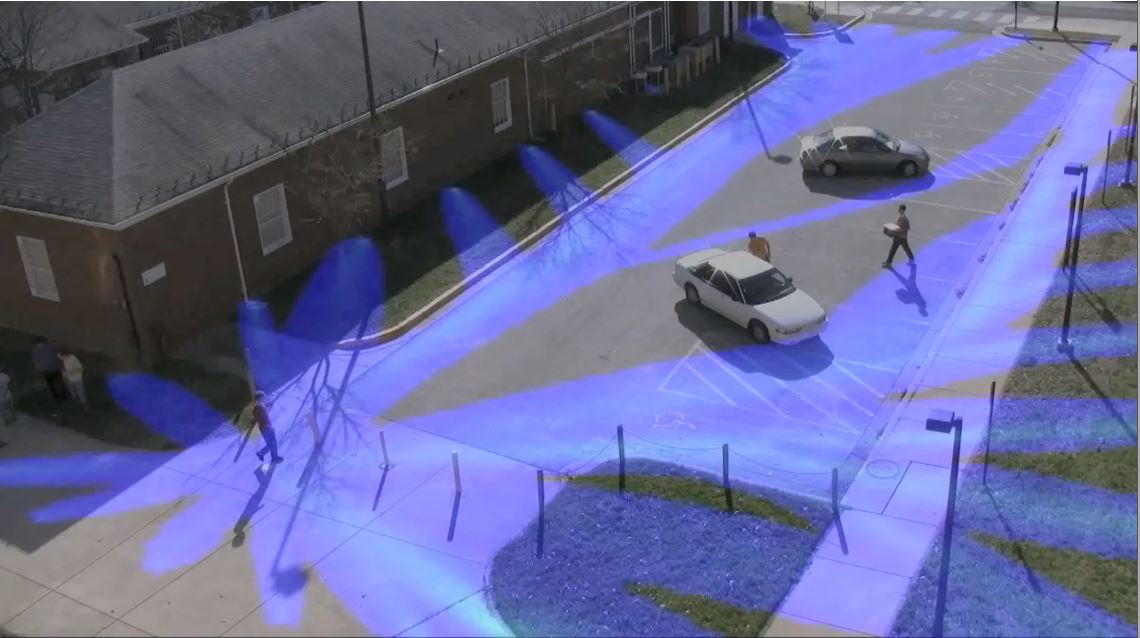
\includegraphics[width=0.8\textwidth]{pic-s3/act-forecast.JPG}
\caption{Activity Forecasting trajectories distribution (Kitani et al, 2012)}
\end{figure}

\subsubsection{Research}
In the research "Activity Forecasting" by Kitani et al (2012), both an expert demonstration and a physical representation of the scene are used to learn a person's decision process, or equivalently, the person's reward function that is not scene specific. The crucial part is that the learned reward function can be generalized to novel scenes. In contrast, if we only learn the trajectory distribution for the parking lot scene, we can only predict trajectory in that one scene, which is not very useful.

\subsubsection{Approach}
In this activity forecasting task, we assume an activity sequence is generated by an Markov Decision Process (MDP) as follow:
\[\zeta = \{x_0, a_0, r(x_0), x_1, a_1, r(x_1),\dots,x_g, a_g, r(x_g)\}\]
\[x_i \in \mathbb{R}^2,\quad a_i \in \mathbb{R}^2,\quad r \in \mathbb{R}\]
where at each time stamp we have a state-action-reward tuple. Each x's represent a 2D coordinate, each a's represent a 2D velocity vector, and each r's is a scalar reward. We model the sequence by a policy:
\[p(a|x) \propto \exp{\{r(x) + \sum_x p(x' | x,a) V(x')\}}\]
The policy is furthered determined by the reward function:
\[V(x) = softmax_a Q(x,a)\]
\[Q(x,a) = r(x) + \sum_{x'} p(x'|x,a) V(x')\]
Put it together, given a reward function, we can compute the value function under MDP. With the value function, we can compute the policy. With the policy, we can sample trajectories from the environment. Although we have this generative process, we have a problem. We only have observations of trajectories, but not the reward function. That is, given a collection of sequences, how do we infer the reward function?

\subsubsection{Reward Function Parameterization}
We solve the problem by parameterizing the reward function with \(theta\):
\[r(x;\theta) = \sum_n \theta_n f_n(x)\]
In the parking lot scene, for example, if we have three features:
\[r(x;\theta) = \theta_{car} f_{car}(x) + \theta_{lot} f_{lot}(x) + \theta_{grass} f_{grass}(x)\]
We can rewrite the reward function with a combination of linear functions over all features. Now the problem is reduced to estimating the \(\theta\)s for each of the features. We can use MaxEnt IRL to do this. The above process is called Inverse Optimal Control

\subsubsection{Key Concepts: IRL under active imitation learning}
\begin{itemize}
    \item IRL can be formulated as a maximum entropy optimization problem
    \item Distribution over trajectories factorizes into a Boltzmann distribution
    \item We can use online mirror descent to solve for reward parameters
\end{itemize}

\subsection{Matrix Game IRL}
Matrix Game IRL demonstrates that a two player game can be solved via online learning. We begin by reviewing the objective function given expert trajectories, assuming trajectories are sample from policy and environment:
\[\zeta^* \sim \pi^* ,\quad \zeta \sim \pi\]
When we compare a policy against the optimal policy, we use the policy value function. The relationship below must hold:
\[V(\pi^*) \geq V(\pi)\]
With the assumption that the reward function can be written as a linear function parameterized by some \(\theta\), we have:
\[\theta \cdot \mu(\pi^*) \geq \theta \cdot \mu(\pi) \]
By moving things around, we have this optimization setup:
\[\min_\theta\{\max_\pi \theta \cdot \mu(\pi) - \theta \cdot \mu(\pi_E)\}\]
where \(\pi_E\) is the expert policy. With more algebra, the objective function is now:
\[\min_\theta\{\max_\pi \theta^T (\mu(\pi) - \mu(\pi_E))\]
\[\theta \in \mathbb{R}^{1 \times N},\quad \mu(\pi) \in \mathbb{R}^{N\times 1}\]
The difference of \(\mu(\pi)\) is the difference in feature counts. We can rewrite this difference with \(G \in \mathbb{R}^{N \times M}\) and \(\psi \in \mathbb{R}^{M \times 1}\):
\[\min_\theta\{\max_\pi \theta^T G \psi\}\]
With \(\theta \in \mathbb{R}^{1 \times N}\), \(G \in \mathbb{R}^{N \times M}\), and \(\psi \in \mathbb{R}^{M \times 1}\) we can now interpret the objective function under the setup of a two players game. We take \(\theta\) as the row player, \(\psi\) as the column player (adversarial), and \(G\) as the matrix game. Note that, we can think \(\psi\) as a mixture of weights over many deterministic policies.

\subsubsection{Online algorithm to solve Matrix Game}
We can solve the matrix game using \hyperref[alg:mwmg]{Multiplicative Weights Algorithm (MWA)} 
\begin{algorithm}
\caption{MW-Matrix Game}
\label{alg:mwmg}
\begin{algorithmic}[1]
\State $\beta$: learning rate
    \Procedure{MW-Matrix Game}{$\beta$}
    \State $w^{(0)} \gets \{w_r^{(0)}=1\}$
    \For{$t=1,\;\cdots,\;T$}
    \State $R^{(t)} = \frac{w^{(t-1)}}{\sum_r w_r^{t-1}}$
    \State $Receive(l^{(t)} = G(\cdot, c^{(t)}))$
    \State $w_r^{(t)} = w_r^{(t-1)} \beta^{l_r^{(t)}} \quad \forall r$
    \EndFor
    \EndProcedure
\end{algorithmic}
\end{algorithm}
Note that inside the for loop at line 5, we are sampling the row player's strategy using a multinomial distribution over the weights, which is similar to the weighted majority algorithm (WMA).

\subsubsection{IRL algorithm to solve Matrix Game}
We can use IRL to solve the matrix game. In the algorithm \hyperref[alg:mwirl]{Multiplicative Weights Inverse Reinforcement Learning Algorithm (MW-IRL)} on line 4-5, we make the prediction based on the current estimated reward function \(\theta\). On line 6, we make update to the reward function estimate.
\begin{algorithm}
\caption{MW-IRL}
\label{alg:mwirl}
\begin{algorithmic}[1]
    \Procedure{MW-IRL}{$\hat{\pi_E}, \hat{\mu_E}, \beta$}
    \For{$t=1,\;\cdots,\;T$}
    \State $\theta_i = \frac{\theta_i}{\sum_{i'} \theta_{i'}} \quad \forall i$
    \State $\hat{\pi_\theta} = RL(r(\cdot; \theta))$
    \State $\hat{\mu} = Estimate(\pi_\theta)$
    \State $\theta_i = \theta_i \cdot \exp{\{\ln{\beta \cdot G_i (\hat{\mu_i})} \}} \quad \forall i$
    \EndFor
    \State \textbf{return} $\theta$
    \EndProcedure
\end{algorithmic}
\end{algorithm}

\subsubsection{Key Concepts: Matrix Game}
\begin{itemize}
    \item Inverse Reinforcement Learning is a two player game between the reward function and a competitive policy
    \item Two player game can be solved with online mirror descent with entropic regularization
\end{itemize}


%\section*{References}
%Include your references here. Please cite any resources you found useful.	
%Populate the refs.bib file or list your references manually. Be consistent in formatting!
{
\bibliography{refs}
\bibliographystyle{abbrv}
}

\end{document} % Done!
